\documentclass[12pt]{article}
\usepackage{tikz}
\usepackage{amsmath}
% Underlining package
\usepackage{ulem}
\usepackage[a4paper, portrait, margin=1cm]{geometry}
\usepackage{fancyhdr}
\usetikzlibrary{calc}

\begin{document}
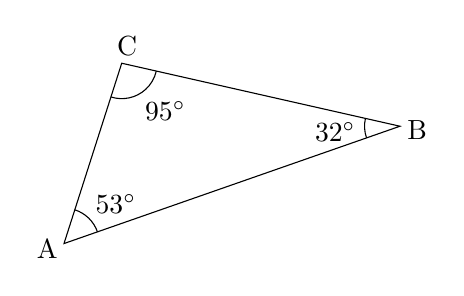
\begin{tikzpicture}[scale=1.5, baseline=(current bounding box.south)]
  \pgfmathsetmacro{\angleA}{int(rnd*40+25)}
  \pgfmathsetmacro{\angleB}{int(rnd*40+25)}
  \pgfmathsetmacro{\sideC}{rnd*1+3}
  \pgfmathsetmacro{\rotationAngle}{rnd*20}
  \pgfmathsetmacro{\angleC}{int(180-\angleA-\angleB)}

  \begin{scope}[rotate=\rotationAngle]
    \coordinate (A) at (0,0);
    \coordinate (B) at (\sideC,0);
    \coordinate (C) at (intersection cs: first line={(A)--($(A)+(\angleA:4cm)$)}, second line={(B)--($(B)+(180-\angleB:4cm)$)});
    \draw (A) -- (B) -- (C) -- cycle;
    
    % Mark angles with arcs
    \draw ($(A)!0.3cm!(B)$) arc [start angle=0, end angle=\angleA, radius=0.3cm];
    \draw ($(B)!0.3cm!(C)$) arc [start angle=180-\angleB, end angle=180, radius=0.3cm];
    \draw ($(C)!0.3cm!(A)$) arc [start angle=180+\angleA, end angle=360-\angleB, radius=0.3cm];
    
    % Label angles
    \node at ($(A)!-0.15cm!(B)$) {A};
    \node at ($(B)!-0.15cm!(C)$) {B};
    \node at ($(C)!-0.15cm!(A)$) {C};
    
    % Mark angles in degrees
    \coordinate (midBC) at ($(B)!0.5!(C)$);
    \node at ($(A)!0.55cm!(midBC)$) {\pgfmathprintnumber{\angleA}$^\circ$};

    \coordinate (midAC) at ($(A)!0.5!(C)$);
    \node at ($(B)!0.55cm!(midAC)$) {\pgfmathprintnumber{\angleB}$^\circ$};

    \coordinate (midAB) at ($(A)!0.5!(B)$);
    \node at ($(C)!0.55cm!(midAB)$) {\pgfmathprintnumber{\angleC}$^\circ$};
 
  \end{scope}
\end{tikzpicture}
\end{document}
